\documentclass[border=10pt]{standalone}
\usepackage{tikz}
\usepackage{pgfplots}
\pgfplotsset{compat=newest}
\usepgfplotslibrary{groupplots}
\usepackage{amsmath}

\begin{document}

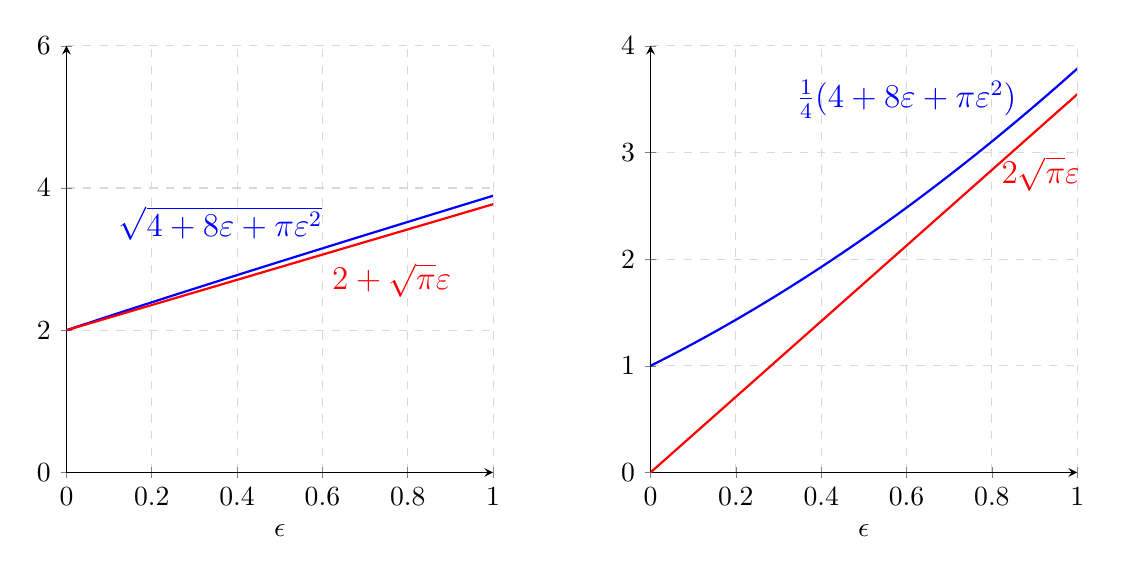
\begin{tikzpicture}
    \begin{groupplot}[
        group style={
            group size=2 by 1, % 1行2列
            horizontal sep=2cm, % 两图之间的间距
            vertical sep=2cm
        },
        width=7cm, height=7cm, % 每张图的大小
        xlabel={$\epsilon$}, % X轴标签
        grid=major, % 显示网格
        major grid style={dashed, gray!30},
        axis lines=left, % 坐标轴样式
        legend pos=north west, % 图例位置
        legend cell align={left},
        xmin=0, xmax=1, % X轴范围 (根据函数形态估算)
        domain=0:3,
        samples=200, % 采样点数,保证曲线平滑
        every axis plot/.append style={thick} % 线条加粗
    ]

    % -----------------------------------------------------------
    % 左侧图表 (Left Plot)
    % -----------------------------------------------------------
    \nextgroupplot[
        ymin=0, ymax=6
    ]
    
    % 蓝色曲线: sqrt(4 + 8e + pi*e^2)
    \addplot[blue, domain=0:1.2, samples=100] {sqrt(4 + 8*x + 3.14159*x^2)};
    % 蓝色文字 (直接放置在图上,模仿截图位置)
    \node[blue, anchor=west] at (axis cs: 0.1, 3.5) {\large $\sqrt{4+8\varepsilon+\pi\varepsilon^2}$};

    % 红色曲线: 2 + sqrt(pi)*e
    \addplot[red, domain=0:1.2, samples=100] {2 + sqrt(3.14159)*x};
    % 红色文字
    \node[red, anchor=west] at (axis cs: 0.6, 2.7) {\large $2+\sqrt{\pi}\varepsilon$};

    % -----------------------------------------------------------
    % 右侧图表 (Right Plot)
    % -----------------------------------------------------------
    \nextgroupplot[
        ymin=0, ymax=4  
    ]
    
    % 蓝色曲线: 1/4(4 + 8e + pi*e^2)
    % 这里使用0.25计算,因为14倍会超出坐标系,且图像显示起点为1
    \addplot[blue, domain=0:1.2, samples=100] {0.25 * (4 + 8*x + 3.14159*x^2)};
    % 蓝色文字
    \node[blue, anchor=center] at (axis cs: 0.6,3.5) {\large $\frac{1}{4}(4+8\varepsilon+\pi\varepsilon^2)$};

    % 红色曲线: 2 * sqrt(pi) * e
    \addplot[red, domain=0:1.2, samples=100] {2 * sqrt(3.14159) * x};
    % 红色文字
    \node[red, anchor=west] at (axis cs: 0.8, 2.8) {\large $2\sqrt{\pi}\varepsilon$};

    \end{groupplot}
\end{tikzpicture}

\end{document}